\section{Introduction}

Many Internet services can benefit from a service that provides a real-time
global view of the state of the network---a {\em traffic map} that can predict
the available bandwidth between a pair of IP
addresses~\cite{clark2003knowledge,madhyastha2006iplane}. For instance, CDNs could implement
better server selection strategies if they could predict Internet path
properties.  Similarly, peer-to-peer applications can be more intelligent in
their choice of peers if they can predict if a specific alternative peer can
offer better performance.  Finally, websites can be optimized to choose
``mirror'' sites  or customize content for their clients if they knew the
network state.  In the absence of such a service, each application  service
provider has  to resort to expensive home-grown solutions or  operate ``in the
dark'' and hope for reasonable performance from the network or simply use
trial-and-error solutions.

 There have been many prior projects that have attempted to tackle some aspects
of this problem; e.g., predicting end-to-end paths~\cite{madhyastha2006iplane} or understanding routing reachability~\cite{katz2008studying} or designing solutions that use
fine-grained measurements to provide deeper insights into the bandwidths and
capacities of individual paths~\cite{pathneck}.  The main challenge that these
past efforts have faced can be captured along three key dimensions: 

\begin{itemize}

\item  {\em Coverage:} Obtaining a global view of the network necessarily entails deploying many millions of 
 vantage points that can run suitable measurement logic to obtain relevant path-level metrics of interest. 
 While recent work  on ``crowdsourcing'' such measurements is indeed promising~\cite{choffnes2010crowdsourcing,sanchez2013dasu,otto2011blind}, even the largest 
 deployed crowdsourced measurement efforts suffer from limited visibility.

\item {\em Overhead:}  While metrics such as reachability or latency are easy to measure,
 the more interesting metrics such as available bandwidth or capacity or the location 
 of bottleneck links have typically required carefully tuned algorithms that  incur 
 non-trivial overhead (e.g., few hundreds of kilobytes per iteration)~\cite{strauss2003measurement}.

\item {\em Real-time views:} This global 
traffic map needs to be updated in near real-time to reflect current network conditions. 
 This raises further concerns in conjunction with the coverage and overhead concerns---we need 
 millions of vantage points continuously running non-trivial measurements {\em all the time.}

\end{itemize} 


\begin{figure*}[t!]
\centering
\subfigure[Client IP prefix (/24)]
{
	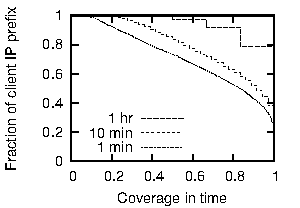
\includegraphics[width=150pt]{data2/cdf-test.pdf}
}
\hspace{-0.5cm}
\subfigure[AS]
{
	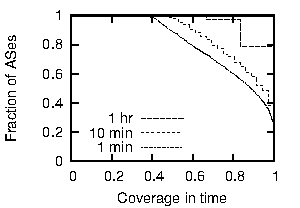
\includegraphics[width=150pt]{data2/cdf-test-clientip.pdf}
}
\hspace{-0.5cm}
\subfigure[ISP]
{
	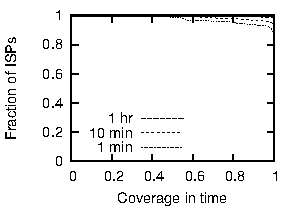
\includegraphics[width=150pt]{data2/cdf-test-isp.pdf}
}
\vspace{-0.2cm}
\tightcaption{Inverse CDF of client-side coverage (fraction of observed client IP prefixes/ASes/ISPs which can be consistently measured) -- Above 94\% of observed ISPs and 36\% of observed ASes can be measured in every minute. }
\label{fig:video:client-coverage}
\end{figure*}

Thus, while the vision of such a global {\em traffic map} for the Internet is
surprisingly simple to state, realizing it has always been out of reach. In
this context, we observe that the growing dominance of Internet video~\cite{interne-traffic-report} and the
ability to instrument video players to collect performance measures of active
video sessions~\cite{de2010experimental}\cite{festive} generates  an unprecedented opportunity to address all
of these aforementioned challenges. Specifically, the dramatic growth of
Internet video provides, for the first time, the capability to obtain real-time
measurements of the network state from millions of vantage points without
incurring any probing overhead!


This paper is a first attempt to outline how we can use video traffic as the
``carrier signal'' that can act as an enabler toward the vision of a real-time
traffic map for the Internet. While the adoption of video does address many of
the challenges, there are still key challenges that remain. First, the
measurement logic  are inherently running in a sandboxed browser or player
environment, meaning that we can only obtain coarse-grained estimates of
observed throughput. Second, we only observe end-to-end path characteristics
between video clients and servers and these may not suffice to cover all links
on the network. 


Fortunately, we show the early promise of addressing these challenges based 
 on two key insights. The first is leveraging the power of a large 
number of measurements from multiple vantage points to compensate for the lack 
of fine-grained measurement from any single vantage point. In some sense, 
 this is analogous to the power of ``big data'' techniques that admit 
 simpler solutions at larger scales~\cite{halevy2009unreasonable}. 
 Second, we find that we do not need a per-link view of the network to 
 effectively answer queries regarding path properties; what we need effectively 
 is only a congestion map that identifies bottleneck links and locating 
 these bottlenecks is easier than estimating the available 
 bandwidth for every link in the network.


In the rest of this paper, we begin by describing the {\em coverage}
opportunities that Interent video as a carrier signal offers based on the views
observed by a single third-party video analytics provider. We outline our
overarching vision for building a video-based traffic map and discuss how we
can address the unique challenges  arising in this context in
Section~\ref{sec:overview}. We  highlight the feasibility of our proposed  in
Section~\ref{sec:ideas}. We discuss outstanding issues in
Section~\ref{sec:disc} before concluding in Section~\ref{sec:concl}.
 We discuss related work inline in the paper.


\comment
{\begin{itemize}
	\item Many applications need network state to inform decisions. 
	\item In spirit of know-plane~\cite{kplane}/iplane~\cite{iplane}, we envision a real time traffic map system as a service that applications can query to obtain information about network states. 
	\item This idea while simple to state has been tantalizingly out of reach. There have been several efforts using different approaches, but never quite satisfying. They cannot do all metrics and they do not provide real time.
	\begin{itemize}
		\item There are several projects (e.g., ~\cite{ningning,iplane}) that assume full control over a few number of vantage points from which the measured performance provides insights of most of the network. Hard to run continuous and simulteneous probing from the vantage points and to claim a representative coverage over the whole network. 
		\item Meanwhile, several other projects proposed to use P2P clients to discover service-level events (\cite{crowdsourcing}) or provide large-scale experiment platforms (\cite{dasu}).
	\end{itemize}
	\item The key challenge has been:
	\begin{itemize} 
		\item Coverage: from client to server-side, from core edge network, from peer-to-peer to client-server(CDN) model, 
		\item Measurement overhead: little additional traffic, non-intrusive instrumentation on client program.
		\item Simultaneous views of the network: critical to localizing network bottleneck.
	\end{itemize}
	\item We observe a never before seen opportunity to address all of these. The key enabler is the streaming video traffic over Internet. It has volume, scale, coverae, and simultaneous views, and in some sense for free. The implication is that it is feasible to measure an unprecedentedly large fraction of Internet in almost real time by measuring one application with little overhead.
	\item In addition, the vision of using video as carrier for a real time internet map leverages other recent trends. (1) More traffic generated by CDN, including streaming video. (2) Embedded measurement code in video player, web page or app -- implication: client-side measurement becomes pervasive. (3) HTTP becomes a converging protocol for data plane of many applications (e.g., web and Internet video) -- implication: application-layer measurement (average throughput and fetching latency) has become equally critical to packet-level information (link latency, packet loss rate).
	\item In this paper, we outline the vision of building a real time service, called Real-time Traffic Map (RTM) -- at any time, anyone can query the current available bandwidth between any two hosts. We present some early feasibility towards such system and outline broader challenges and opportunities.
\end{itemize}
}
